

%\begin{flushright}
%  {\em QUOTE GOES HERE }\\
%
%\ \
%
%\normalsize
%{AUTHOR}  
%\end{flushright}
\chapter{Probing DAMOCLES:  Testing and a Parameter Sensitivity Analysis}\label{chp:chp4}

The introduction of any new piece of software into a field has the potential to yield exciting new results.  The first step in this process should therefore be a thorough investigation into the reliability of the code and an assessment of the outputs from a theoretical standpoint.  Before the modelling of real data takes place, it is important to understand why the variation of a  given parameter affects results in a particular way.  A comprehensive understanding of parameter space not only facilitates the modelling process but may also give rise to interesting results in and of itself.

To this end, this chapter describes the ways in which DAMOCLES was tested and the results of these tests.  I then also present a parameter sensitivity analysis.  I describe the changes that are seen in the shapes of line profiles and consider any distinctive features that arise as a result of varying the parameters of interest.  I also contemplate the physical processes behind these effects.


\section{Testing and benchmarking the code}

The field of astronomy is highly reliant on the production of bespoke software to understand and interpret observations from telescopes and to develop and test new theories.  As one of only a few sciences which do not have the ability to run experiments or to validate results in a laboratory, progress is made via mathematical analyses or computational models based on observed data.  Astrophysicists typically develop their own programs because a deep understanding of the topic to be modelled is required.  Like any experiment, however, the ``apparatus" should be checked and tested in order to establish its reliability.

Throughout the production of DAMOCLES, I sought, as far as was possible, to maintain best practices in scientific computing as detailed by \citet{Wilson2012}.  The code is carefully structured into modules and subroutines as described in the previous chapter.  Each of these units was inspected for sense and accuracy as it was written, and at each update and addition the code as a whole was tested against basic logical checks, for example comparing outputs to manually calculated properties.  In addition to regular evaluations conducted throughout the program development, it was very important to establish that DAMOCLES produced standard results as expected.

There is a general lack of published models in the literature that consider dust-affected asymmetric line profiles.  This is problematic since there are no published benchmark cases against which I could compare results.  I therefore considered a number of analytic line profiles derived from first principles for the case of a dust-free spherically symmetric expanding medium.  This process ensured the functionality of the grid and the initialisation and propagation of energy packets.  Additionally, I also checked the the absorption and scattering components of the code which are crucial to the modelling of a dusty medium.  I  considered some optically thick scenarios and qualitatively compared my results with those derived by \citet{Lucy1989}.  The profiles presented by  \citet{Lucy1989} are produced both analytically and from numerical modelling and are of scenarios that are typical of those treated by DAMOCLES.  They are also the only published numerical models of dust-affected asymmetric line profiles and as such it is important that DAMOCLES is capable of reproducing these results.

\subsection{Theoretical line profiles from first principles}
\label{analytics}

The simple nature of a spherically-symmetric expanding medium with a given velocity outflow law and emissivity distribution allows for analytical line profiles to be calculated from first principles in the dust-free case.  Based on the methods of \cite{Gerasimovic1933},  I derive a set of three equations that describe the contours of theoretical line profiles under different starting conditions.



Describing the fractional expansion velocity of the shell as $v(r) \propto 
r^\alpha$ with $\alpha \neq 0$ such that $v(r)=\frac{V(r)}{V_{max}}$ where 
$V(r)$ and $V_{max}$ represent physical velocities and $v_{max}=1$, the velocity along the line-of-sight to the observer is given by 
\begin{equation}
\label{eqn:radial_vel}
u(r,\theta)=r^\alpha \cos \theta
\end{equation}

\noindent For curves with constant line-of-sight velocity $u=const$ we therefore have
\begin{equation}
\,d r = \frac{r}{\alpha} \tan \theta \,d \theta
\end{equation}

\begin{figure}
\includegraphics[clip=true,scale=0.5,trim= 180 50 130 70]{chapters/chapter4/images/opt_thin_diag/curve.png}
\includegraphics[clip=true,scale=0.5,trim= 180 50 130 70]{chapters/chapter4/images/opt_thin_diag/line.png}
\caption{Diagrams illustrating the dust-free model and some of the relevant variables used in the derivation of the equations of analytical line profiles.  On the left is the general case with curves of constant $u$ labelled.  On the right is the special case of an orthogonal $(u,s)$ net when $\alpha=1$ and therefore $v(r) \propto r$.}
\label{fig:analytics}
\end{figure}


\noindent For $u=const$, the line element $\, ds$  is given by
\begin{equation}
\label{eqn:ds}
\, ds^2 = r^2 \, d\theta^2 + \, dr^2 = r^2 \Big( \frac{\tan^2\theta}{\alpha^2}+1 \Big)\, d\theta^2
\end{equation}

\noindent and therefore, along curves of constant $u$ we have
 \begin{equation}
 \label{eqn:vs}
s = u^{\frac{1}{\alpha}} \int_{\theta_{0}}^{\theta_{1}} \frac{\sqrt{\frac{\tan^2\theta}{\alpha^2}+1}}{\cos ^ {\frac{1}{\alpha}}\theta}\, d\theta
\end{equation}


\noindent The angle $\psi$ between the tangent to a curve and the radial line  is given by the formula (in polar coordinates) \begin{equation}
\tan \psi = r \frac{\, d \theta}{\, d r} 
\end{equation}

\noindent which for curves of $u=const$ gives
\begin{equation}
\tan \psi = \frac{\alpha}{\tan \theta}
\end{equation}

Curves of constant line-of-sight velocity therefore intersect the line $\theta = 0$ orthogonally, although the $(u,s)$ net is only orthogonal if $\alpha=1$ (see Figure \ref{fig:analytics}).

We can now construct a volume element between $u$ and $u+\, du$ by rotating a section of thickness $\, du$  around the $\theta =0 $ axis.  Assuming that $i(r)$ is the emission per unit volume (dependent only on radius), then the energy emitted by the nebula between $u$ and $u+du$ is proportional to
\begin{equation}
\label{eqn:integral}
\int_{\mathcal{C}} \ i(r) \ r \sin \theta \ r \, d\theta \, dr  \ = \ \int_{\mathcal{C'}} \ [i(r) \ r^2 \sin \theta] \ \frac{\partial (r,\theta)}{\partial (u,s)}  \, ds \, du
\end{equation}

where the integral is a line integral along curves $\mathcal{C}$ of constant $u$ and square brackets denote a change of variables.  

We therefore compute the Jacobian from Equations \ref{eqn:radial_vel} and \ref{eqn:vs} as
\begin{equation}
\label{eqn:jacob}
\frac{\partial (u,s)}{\partial (r,\theta)} \ = \ \alpha  u \sqrt{\frac{\tan^2\theta}{\alpha^2}+1}
\end{equation}

Assuming an initial emissivity distribution dependent on radius only, we put $i(r) \propto r^{-2\beta}$ (i.e. appropriate for a gas density distribution $\rho \propto r^{-\beta}$ with the emissivity proportional to the gas density squared).  Substituting Equation \ref{eqn:jacob} into Equation \ref{eqn:ds} and calculating the curvilinear integral along curves of constant $u$ yields the following:
\begin{equation}
i(u) \,d u \ \sim \, du \int_\mathcal{C} \frac{r^{2(1-\beta)}\sin \theta}{\alpha u \sqrt{\frac{\tan^2\theta}{\alpha^2}+1}} \, ds 
\end{equation}

Substituting in Equations \ref{eqn:radial_vel} and \ref{eqn:integral} and transforming to an integral in $\theta$ gives
\begin{equation}
\begin{split}
i(u) \, du &\sim \frac{du}{\alpha u^{\frac{2\beta-3+\alpha}{\alpha}}} \int^{\theta_1}_{\theta_0} \cos^{\frac{2\beta-3}{\alpha}} \theta \sin \theta \, d\theta 
\\
&\sim  \frac{du}{u^{\frac{2\beta-3+\alpha}{\alpha}}} \Bigg[\frac{\cos^{\frac{2\beta - 3 + \alpha}{\alpha}} \theta}{2\beta -3 + \alpha}\Bigg]^{\theta_1}_{\theta_0}
\end{split}
\end{equation}

\noindent for $\frac{2\beta-3}{\alpha} \neq -1$ where $i(u) \,du$ is the energy emitted in a volume element and $\theta_0$ and $\theta_1$ are the bounds of this element.  The case $\frac{2\beta-3}{\alpha} = -1$ results in a logarithmic relationship.

\begin{figure}
\begin{subfigure}{0.5\textwidth}
\centering
\includegraphics[trim =0 25 45 15,clip=true,scale=0.4]{chapters/chapter4/images/params/A/b0_r0_2}
\end{subfigure}
\hspace{4mm}
\begin{subfigure}{0.5\textwidth}
\centering
\includegraphics[trim =72 25 45 15,clip=true,scale=0.4]{chapters/chapter4/images/params/A/b0_r0}  
\end{subfigure} \\[0.0ex]

\begin{subfigure}{0.5\textwidth}
\centering
\includegraphics[trim =0 25 45 15,clip=true,scale=0.4]{chapters/chapter4/images/params/A/b1_r0_2}
\end{subfigure}
\hspace{4mm}
\begin{subfigure}{0.5\textwidth}
\centering
\includegraphics[trim =72 27 45 15,clip=true,scale=0.4]{chapters/chapter4/images/params/A/b1_r0} 
\end{subfigure} \\[1.0ex]

\begin{subfigure}{0.5\textwidth}
\centering
\includegraphics[trim =0 0 45 15,clip=true,scale=0.4]{chapters/chapter4/images/params/A/b2_r0_2}
\end{subfigure}
\hspace{4mm}
\begin{subfigure}{0.5\textwidth}
\centering
\includegraphics[trim =72 0 45 15,clip=true,scale=0.4]{chapters/chapter4/images/params/A/b2_r0.pdf}
\end{subfigure}

\caption{\textit{Red:} Benchmark models for optically thin ($\tau =0$) 
line profiles  with fractional velocity $v(r) \propto r$. Top to bottom: initial emissivity 
profiles $i(r) \propto r^{-2\beta}$ with $\beta=0.0$, $\beta=1.0$ and 
$\beta=2.0$. Cases with $R_{in}/R_{out}=0.2$ are on the left and 
$R_{in}/R_{out}=0.0$ on the right.  The presence of a plateau in the upper plots is due to the finite inner radius (detached shell). \textit{Blue:} The analytical case 
with $i(u) \sim 1-u^{2(1-\beta)}$ except in the case of $\beta=1$ where 
$i(u) \sim -\log u$.}
\label{fig:analytics}
\end{figure}



In the case of a ``filled'' nebula, i.e. one where the inner radius is vanishingly small in comparison to the outer radius the above result may be evaluated between $\theta_0=0$ and $\theta_1=\arccos u$ and the equation of the line profile is
\begin{equation}
\label{eqn:sides}
	i(u) \, du \sim \pm \frac{du}{(2\beta-3+\alpha) u^{\frac{2\beta-1+\alpha}{\alpha}}} \Big(1-u^{\frac{2\beta-3+\alpha}{\alpha}} \Big)
\end{equation}

If the nebula is not ``filled'', that is to say, the inner radius is some fraction of the outer radius and the remnant is a detached shell  with inner radius $R_{in}=q$ and outer radius $R_{out}=1$ such that $q=\frac{R_{in}}{R_{out}}$, the 
above formula is only valid from some critical value $u'=q^{\alpha}$ to $u=1$. For $u<u'$, we obtain
\begin{equation}
i(u) \, du \sim \pm \frac{du}{(2\beta-3+\alpha)} \Big( \frac{1}{q^\alpha} - 1 \Big)
\end{equation}

\noindent and therefore the top of the line is flat while the sides are 
sloping.

Crucially, the width of the flat section is determined by 
\begin{equation}
\label{eqn:flattop}
u'=q^{\alpha}
\end{equation} 

\noindent or simply $u'=q$ in the case where $v \propto r$, whilst the shape of the profile outside of the flat-topped region is described by Equation  \ref{eqn:sides}.

Profiles with a variety of shapes may be derived from these formulae  depending on the relative values of $\alpha$ and $\beta$.  Here we consider three main families of curves:


\begin{enumerate}\parskip3pt

	\item \ \ $\quad i(u)  \sim u^{-\gamma}-1$ \quad ($\alpha>0$, $2\beta-3+\alpha>0$)
	\item \ $\quad i(u)  \sim 1-u^\gamma$ \quad \ \ ($\alpha>0$, $2\beta-3+\alpha<0$)
	\item  $\quad i(u) \sim -\log u$ \quad \ \ ($\alpha>0$, $2\beta-3+\alpha=0$)

\end{enumerate}

\begin{figure}
\centering
\includegraphics[trim =0 0 0 0,clip=true,scale=0.6]{chapters/chapter4/images/Lucy89_Model2.png}
\caption{The analytically derived line profiles of \citep{Lucy1989} corresponding to their Model II scenario with zero albedo dust for a variety of total dust optical depths.}
\label{fig:LucyMod2}
\end{figure}

\noindent where $\gamma$ is defined as $\gamma= \lvert 
\frac{2\beta-3+\alpha}{\alpha} \rvert$.

Models are presented for each of these cases, both for a filled nebula and for a shell structure with $R_{in}/R_{out}=0.2$.  A velocity profile $v \propto r$ appropriate for supernova ejecta in the free expansion phase is used throughout \citep{Li1992,Xu1992,McCray1996,Baron2005}.  Values of 
$\beta = 0, 1$ and $2$ are adopted.  Figure \ref{fig:analytics} 
illustrates the excellent agreement between the analytical case and the 
models.  All fluxes are scaled to unity at the peak.

I conclude from this testing that all aspects of the code that are associated with initialising the packets into the grid are functioning correctly since an error at this stage would result in disagreement with the above theory.  

\subsection{Comparison of DAMOCLES models with previously published results}
\label{opt_thick_testing}
\begin{figure}
\centering
\includegraphics[trim =0 0 0 0,clip=true,scale=0.6]{chapters/chapter4/images/Lucy89_Model3.png}
\caption{The numerically modelled line profiles of \citep{Lucy1989} corresponding to their Model III scenario with dust of albedo $\omega=0.6$ for a variety of total dust optical depths.}
\label{fig:LucyMod3}
\end{figure}



In addition to the tests for the optically thin line profiles detailed above, I also compared my outputs to those derived by \citet{Lucy1989} in order to assess the accuracy of the scattering and absorption aspects of the code.  
I  considered two similar cases, equivalent to Models II and III of 
\citet{Lucy1989} (see Figures \ref{fig:LucyMod2} and \ref{fig:LucyMod3} respectively). In the first case, dust with zero albedo (pure absorption) was 
uniformly distributed throughout a filled nebula with a velocity profile 
$v \propto r$.  In the second case, the same scenario was considered but in a 
medium of dust with albedo $\omega =0.6$.

In the first case, the profile may once again be derived analytically from 
the basic geometry using the fact that radiation will be attenuated by a 
factor $e^{-2\tau_{\nu} v}$ between points with line-of-sight fractional 
velocities $-v$ and $+v$ where $\tau_{\nu}$ is the optical depth at 
frequency $\nu$ from the centre to the outer edge of the ejecta.  The line 
profile is therefore given by
\begin{equation}
\frac{I(v)}{I(-v)} = \exp(-2\tau_{\nu} v)  
\end{equation}
\begin{figure}
\begin{subfigure}{\textwidth}
\centering
\includegraphics[trim =10 0 45 15,clip=true,scale=0.67]{chapters/chapter4/images/params/opt_thick_w0}
\end{subfigure} \\[1ex]
\begin{subfigure}{\textwidth} 
\centering
\includegraphics[trim =10 0 45 15,clip=true,scale=0.67]{chapters/chapter4/images/params/opt_thick_w0_6}
\end{subfigure}  
\caption{Benchmark models for line profiles  with $v \propto r$, $i(r) \propto$ constant and a filled sphere with $R_{in}/R_{out}=0$.  Pure dust absorption models ($\omega = 0$) are presented in the top plot, whilst partially scattering models are presented at the bottom ($\omega = 0.6$) as per \citet{Lucy1989} Models II and III. All resulting profiles have been scaled to unity flux at their peaks.}
\label{fig:Lucy}
\end{figure}


\citet{Lucy1989} presented several examples for both the analytical case of 
the perfect absorber and a Monte Carlo model for grains with albedo $\omega 
=0.6$.  I include their profiles here for comparison in Figures \ref{fig:LucyMod2} and \ref{fig:LucyMod3}.  I  present line profiles in Figure \ref{fig:Lucy} that were generated by DAMOCLES using the same model parameters as described by \citet{Lucy1989}.  I note that 
the resulting profiles exhibit the same features and shape. The peak of all profiles is shifted further to the blue with increasing optical depth and all profiles are also flux-biased towards the blue.  Of particular 
interest is the scattering wing that appears beyond the maximum velocity 
($v_{max}=1$) on the red side of the profiles in the partial 
scatterer case as a result of the packets doing work on the expanding sphere.  
This was noted by \citet{Lucy1989} as a potential diagnostic for the 
presence of dust in the ejecta of a supernova and I  will discuss this 
further in the next section.


%\subsection{Testing the electron scattering mechanism}
%\subsection{Clumped models in smooth limits}


%%%%%%%%%%%%%%%%%%%%%%%%%%
\section{A Parameter Sensitivity Analysis}
It is of general interest to establish potential diagnostic signatures in 
the line profiles of supernovae and their remnants in order to trace dust 
formation more effectively. The capacity to specify a number of parameters is included in DAMOCLES.  The variation of each parameter potentially affects the contour of the resulting line profile in a different way.  By investigating each parameter separately over a range of values whilst keeping the other parameters fixed, it may be possible to identify certain characteristics of dust-affected line profiles that may be associated with a particular property of the dusty medium.  This insight could help to explain unusual or interesting features of observed line profiles where dust is suspected to be an influential factor.  In this chapter, I investigate and discuss the effects of the main 
parameters of interest, namely:

\begin{itemize}
\item the maximum velocity, $V_{max}$
\item the ejecta radius ratio, $R_{in}/R_{out}$
\item the dust optical depth,  $\tau$
\item the dust albedo, $\omega$ 
\item the dust density profile exponent, $\beta$, where $\rho \propto r^{-\beta}$
\end{itemize}

I also investigate the capacity of this type of model to infer properties of the dust itself, specifically the dust grain radius range and distribution, and the variety and relative abundances of different species present in the dusty medium. 


\subsection{The maximum line velocity, $V_{max}$}

The maximum velocity is defined as the velocity at the outer edges of the 
line emitting region for a given line.  The maximum velocity may vary 
between different spectral lines or doublets due to different locations of 
species having differing ionization thresholds.  Clearly, the larger the 
maximum velocity used the wider the profile becomes.  To some extent 
therefore the steepness of the density profile and the maximum velocity 
can act to counter each other since a steeper density distribution narrows 
the profile (see Section \ref{beta}).  The shape of the wings of the 
profiles, however, generally precludes much degeneracy in this aspect - the 
overall shape of the line profile can be used to determine the exponent of 
the density distribution to within a relatively small range.

More important is the effect that the maximum velocity has on the overall 
optical depth.  Since the outer radius is calculated directly from the 
maximum velocity (as $R_{out}=V_{max} \times t$ where $V_{max}$ is determined from the blue side of the observed line profile), the overall volume of the ejecta is determined solely by 
this value and the ratio of the inner and outer radii.  The total dust 
optical depth to which the radiation is exposed can therefore be greatly 
affected by even a relatively small change in the maximum velocity for 
fixed values of the other parameters.  Practically, however, the maximum 
velocity can usually be fairly well determined from the observations 
(identified as the point where the flux vanishes on the blue side) and may 
be further constrained through modelling.

\subsection{The ejecta radius ratio, $R_{in}/R_{out}$}

As already discussed in Section \ref{analytics}, the width of the flat top 
is determined by the ratio of the inner and outer radii, the exponent of 
the velocity profile and the maximum velocity.  I assume that the 
supernova is in free expansion from just a few months after the explosion 
and therefore $r=vt$ such that within the ejecta the velocity profile 
takes the form $v \propto r$ at a fixed time i.e. the supernova expands 
self-similarly \citep{Li1992,Xu1992,Kozma1998b}.  For this case, 
$R_{in}/R_{out}$ is given by

\begin{equation}
\frac{R_{in}}{R_{out}}=\frac{V_{min}}{V_{max}}
\end{equation}

\noindent where it is often possible to constrain $V_{min}$ and $V_{max}$ 
to a relatively narrow range simply from the observed line profile.

The majority of spectral lines emitted from supernovae and supernova 
remnants are expected to have a flat top before dust attenuation effects 
since it is rare for these objects to form a completely filled nebula.  
However, even a very small amount of dust attenuation may result in the 
line profile appearing to be smoothed at its peak.

The effects of absorption by dust on a line profile for a filled nebula 
with $R_{in}/R_{out}=0$, as opposed to a detached shell, are shown in 
Figure \ref{fig:Lucy}. 
All profiles have been scaled to unit flux at their peaks.

\subsection{The dust optical depth, $\tau$}
\label{tau}

As expected, greater attenuation of the original line profile is seen on 
the red side (see Figures \ref{wt} and \ref{bt} ).  The profiles are most 
revealing at lower dust optical depths since the effects of the asymmetric 
absorption can be seen in different sections of the profiles and the 
profiles therefore tend to exhibit more features. The region of the 
profile that is most clearly affected by dust absorption is the 
flat-topped region.  A small amount of absorption in this region results 
in a skewed profile, with a fraction of the flat-topped section removed.  
The peak becomes blue-shifted as a result, but only to the original value 
of $-V_{min}$, the minimum velocity corresponding to $R_{in}$. In addition 
to the attenuation in this region, the red wing of the profile is also 
somewhat reduced, and the blue wing somewhat increased relative to their 
original symmetric positions.  The result is a relatively ``jagged'' 
looking profile, often with sharp changes at $\pm V_{min}$.  The profile 
is generally asymmetric, although the degree of absorption in the 
flat-topped region may sometimes make it seem as though the profile is in 
fact symmetric and uniformly blue-shifted (see Section \ref{asym} for 
further discussion).  Observationally, these sharp features might become 
smoothed due to insufficient spectral resolution.

At high dust optical depths or when the ratio of the inner and outer radii 
is small, the entire profile is shifted to the blue and the peak moves 
beyond $-V_{min}$ further into the blue.  The profiles also tend to become 
more smooth and featureless.  A set of models showing the effects of 
varying optical depths for different density profiles and dust albedos are 
presented in Figures \ref{wt} and \ref{bt} with $R_{in}/R_{out} = 0.2$.

\begin{figure}
\centering
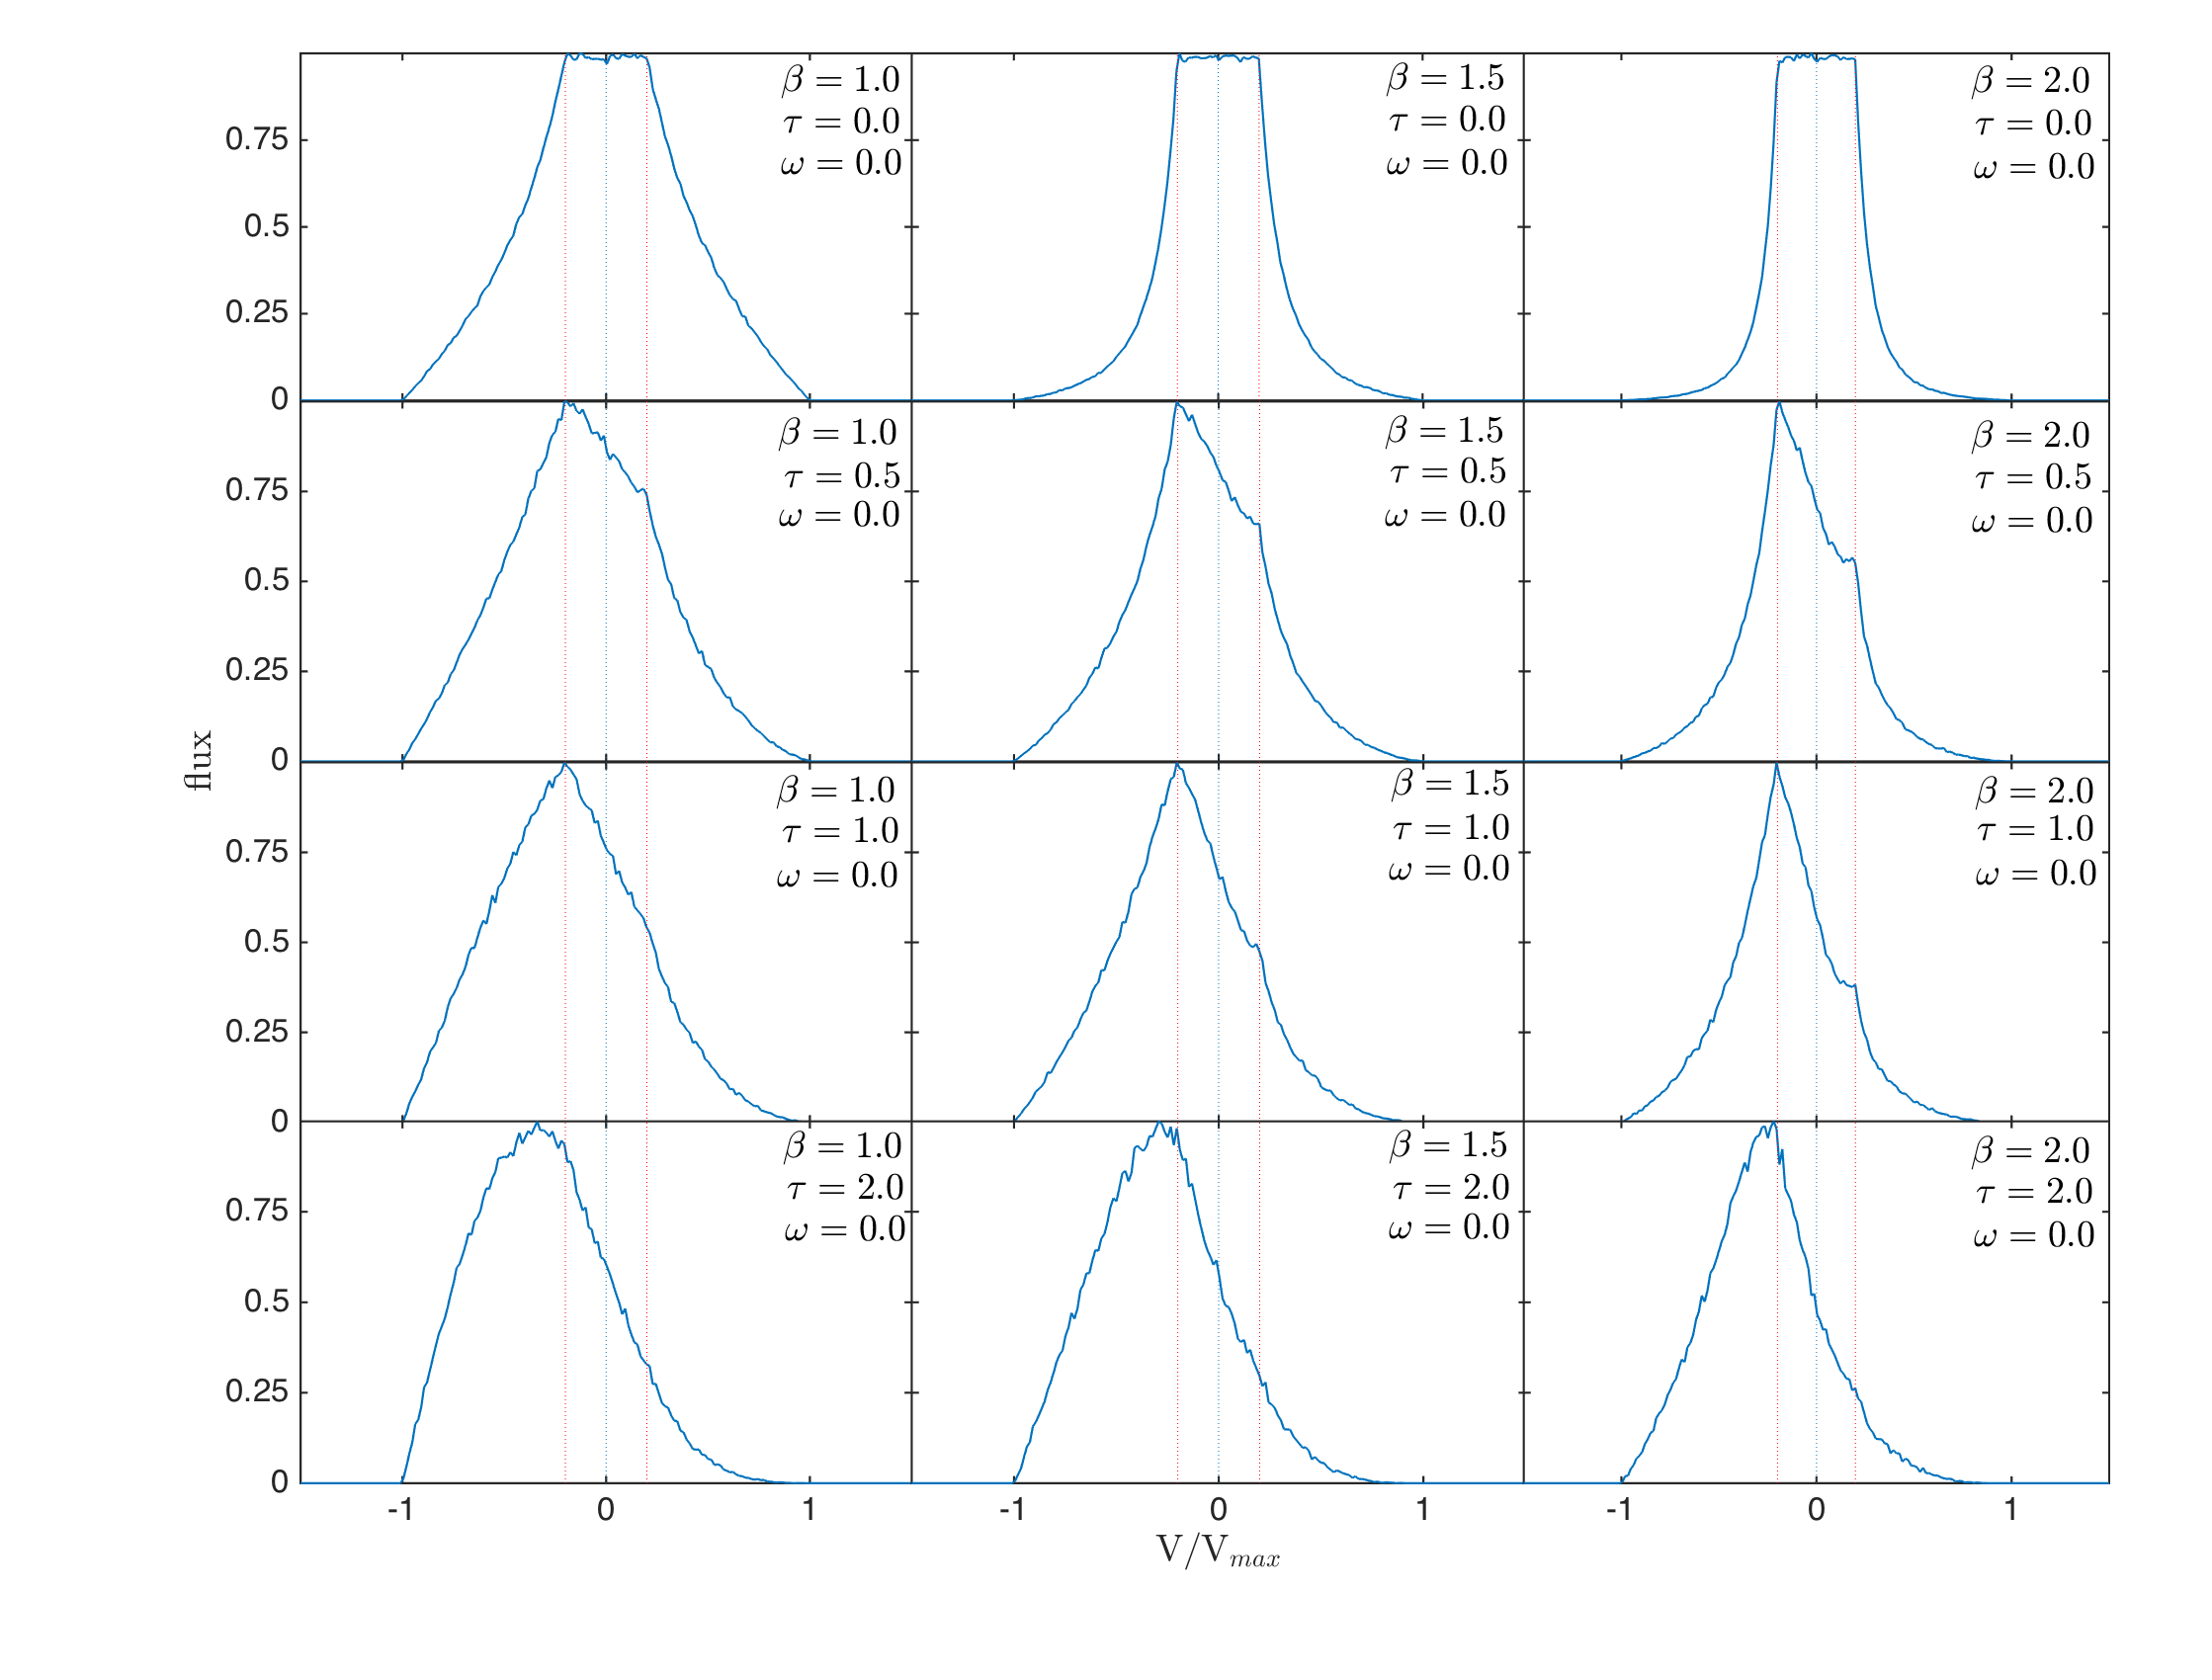
\includegraphics[trim =77 0 6 15,clip=true,scale=0.44]{chapters/chapter4/images/params/D/D_all}
\caption{Set of models with $i(r) \propto r^{-2\beta}$ for $\beta=1.0$ (left), $\beta=1.5$ (middle) or $\beta=2.0$ (right), $\omega=0$, 
$R_{in}/R_{out}=0.2$, $v(r) \propto r$ and $v_{max}=1$ illustrating the effects of varying 
$\tau$.  Peak fluxes are scaled to unity.}
\label{bt}
\end{figure}


%At high dust optical depths or when the ratio of the inner and outer radii 
%is small, the entire profile is shifted to the blue and the peak moves 
%beyond $-V_{min}$ further into the blue.  The profiles also tend to become 
%more smooth and featureless.  A set of models showing the effects of 
%varying optical depths for different density profiles and dust albedos are 
%presented in Figures \ref{wt} and \ref{bt} with $R_{in}/R_{out} = 0.2$.



\subsubsection{The complete nebula case}

To reproduce similar characteristic dust-affected line profiles where the peak of the profile is shifted beyond $-V_{min}$ into the blue is ``easier" for smaller values of $V_{min}$.  The complete nebula is therefore effectively analogous to cases of higher optical depths for a detached shell and the same effects that are illustrated in Figures \ref{bt} and \ref{wt} apply.

%NEED MORE HERE - PRESENT A MODEL?

\begin{figure}
\centering
\includegraphics[trim =70 40 40 15,clip=true,scale=0.43]{chapters/chapter4/images/params/C/C_all}
\caption{Set of models with $i(r) \propto r^{-4}$ (i.e. $\beta=2.0$), $R_{in}/R_{out}=0.2$, $v(r) \propto r$  
and $v_{max}=1$ illustrating the effects of varying $\tau$ and $\omega$. 
Peak fluxes are scaled to unity.}
\label{wt}
\end{figure}


\subsection{The dust albedo, $\omega$}
\label{omega}

In the past, there has often been a focus on the effects of absorption by 
dust on the shapes of line profiles and less attention has been paid to 
the potential effects of scattering by dust.  In fact, line profiles can 
be significantly affected by scattering of radiation.  The greater 
attenuation of radiation received from the receding portion of the ejecta 
results in an asymmetry of the line profile whereby the majority of the 
observed emission is located bluewards of the peak.  However, the effects 
of repeated dust scattering events within the ejecta can substantially 
alter the shape of a line profile and potentially can act to counter the 
blue-shifted asymmetry.

Not only does repeated scattering of photons increase the number of 
potential opportunities for a given photon to be absorbed but it also 
results in continuous shifting of the frequency of the photon to the red.  
The photon must do work on the expanding shell of dust in order to escape 
and thus many of the photons are reprocessed beyond the theoretical 
maximum velocity on the red side of the profile.  Even in the case of dust 
grains with a relatively low albedo, a surprisingly persistent wing on the 
red side of the profile is seen, generally beyond the maximum theoretical 
velocity of the emitting region. In the case of strong dust scattering and 
high dust optical depths, this can actively result in a shift in the 
overall asymmetry of the profile, with the majority of the emission being 
emitted redwards of the peak. The peak however, remains blue-shifted (for 
example the bottom left panel of Figure \ref{wt}) or central (for example 
the bottom right panel of Figure \ref{wt}).  For the line profile to 
exhibit this effect requires the dust to be a nearly perfect scatterer;
of the albedos plotted in Figure \ref{albedo_grain}
only the nearly-transparent MgSiO$_3$ sample of \citet{Jager2003}
exhibits such a behaviour.

The combination of relatively low dust optical depths, initially 
flat-topped profiles, greater attenuation on the blue side along with 
increased flux on the red side due to scattering can result in a profile 
that sometimes ends up appearing almost symmetrical, particularly if 
contaminants, such as narrow lines or blending with other broad lines, are 
present or if the resolution of the data is low.  The potential for 
apparently symmetrical profiles that appear to have been uniformly 
blue-shifted should be noted (see Figures \ref{wt} and \ref{bt} for 
examples of this).


\subsection{The dust density profile, $\rho \propto r^{-2\beta}$}
\label{beta}

Whilst the density profile of the dust may have some effect on the 
resulting profiles, it is the initial emissivity profile (dependent on the 
gas density profile) that has the greatest effect on the shape of the line 
profile.  In general, the steeper the emissivity distribution, the 
narrower the line profile becomes.  The sides of the line profile may 
become almost vertical for a very steep distribution since the majority of 
the emission then comes from a very narrow velocity range (see Figure 
\ref{fig:analytics}).  For a flat-topped profile of 
fixed width this approximates the square profile produced in the case of 
an emitting shell with constant velocity.

\begin{figure}

\begin{subfigure}{1\textwidth}
\centering
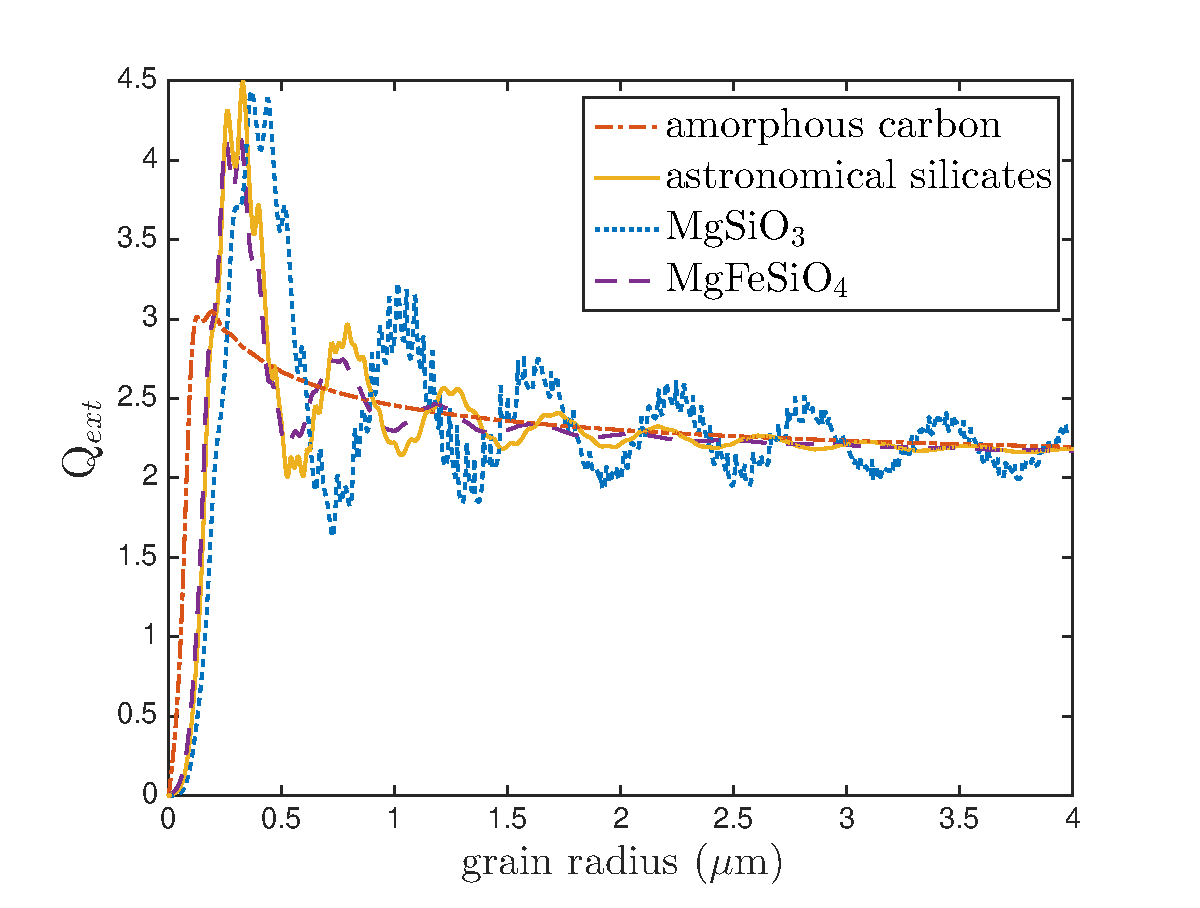
\includegraphics[trim =20 0 45 15,clip=true,scale=0.7]{chapters/chapter4/images/Qext_grainsize_upto4}
\end{subfigure}\\[1ex]
\begin{subfigure}{\textwidth}
\centering
\includegraphics[trim =20 0 45 15,clip=true,scale=0.7]{chapters/chapter4/images/Qext_grainsize_upto4_log}
\end{subfigure}
\caption{The variation of extinction efficiency ($Q_{ext}$) 
with grain radius at $\lambda$ =  656~nm for \citet{Zubko1996} BE amorphous 
carbon, \citet{Draine1984} astronomical silicate and the
MgSiO$_3$ and MgFeSiO$_4$ samples of \citet{Jager2003} and 
\citet{Dorschner1995} respectively. A linear scale is presented on the top and a log scale on the bottom.}
\label{Qext_grain}
\end{figure}

\begin{figure}
\begin{subfigure}{1\textwidth}
\centering
\includegraphics[trim =20 0 45 15,clip=true,scale=0.7]{chapters/chapter4/images/albedo_grainsize_upto4}
\end{subfigure}\\[1ex]
\begin{subfigure}{1\textwidth}
\centering
\includegraphics[trim =20 0 45 15,clip=true,scale=0.7]{chapters/chapter4/images/albedo_grainsize_upto4_log}
\end{subfigure}
\caption{The variation of albedo with grain radius at $\lambda$ =  656~nm for \citet{Zubko1996} BE amorphous 
carbon, \citet{Draine1984} astronomical silicate and the
MgSiO$_3$ and MgFeSiO$_4$ samples of \citet{Jager2003} and 
\citet{Dorschner1995} respectively. A linear scale is presented on the top and a log scale on the bottom.}
\label{albedo_grain}
\end{figure}

The dependence of the shape of the line profile on the emissivity 
distribution is described analytically in Section \ref{analytics} for the 
case of very optically thin dust.  However, for even fairly low dust 
optical depths, the density profile plays a significant role in 
determining the shape of the line profile where it is affected by dust 
absorption.  As previously discussed, at relatively small optical depths 
for reasonable $R_{in}/R_{out}$, a section of the flat-topped region is 
removed resulting in a peak at $-V_{min}$.  The shape of the profile in 
this region is significantly affected by the density profile.  Shallow 
density profiles (low $\beta$) produce a virtually linear variation in 
flux between $-V_{min}$ and $+V_{min}$ (for example the profiles in the 
left column of Figure \ref{bt}).  For a fixed dust optical depth, the 
steeper the distribution becomes, the more concave the profile becomes 
between $-V_{min}$ and $+V_{min}$, ultimately resulting in a clear 
shoulder to the profile at $+V_{min}$ (for example the profiles in the 
right column of Figure \ref{bt}).  For extremely steep density 
distributions this can result in a double peaked profile with a trough to 
the red of $V=0$.  An illustration of the effects on the line profiles of 
varying $\beta$ and $\tau$ is shown in Figure \ref{bt}.  As previously 
noted, these features may not be apparent in observed line profiles with 
poor spectral resolution.

\subsection{Inferring properties of the dust from the models}

The presence of an extended red wing at large positive velocities in 
combination with increased extinction on the red side at smaller positive 
velocities can allow the values of $\tau$ and $\omega$ to be well 
constrained.  Where this occurs it is possible to translate these values into a 
dust mass and grain radius for a given species or combination of 
species using grain optical properties and Mie theory (see Figure 
\ref{albedo_grain}).  


For amorphous carbon, the albedo generally increases with grain radius.  
The presence and extent of any scattering wing on the red side of the 
observed profile can therefore help to place limits on the grain radius.  
However, the greater the grain radius used the smaller the available 
cross-section for interaction per unit dust mass.  Larger masses of dust 
are therefore required to fit the same degree of absorption if a larger 
grain radius is used.  This is in contrast to SED radiative transfer 
modelling where larger grain radii generally result in less dust being 
required to fit the IR portion of the SED (W15).  These two techniques in 
tandem may therefore provide limits on grain radii for different species 
or combinations thereof.

It is known that the use of different optical properties may substantially 
alter dust masses derived using SED fitting for a given species of 
specific grain radius (e.g. \citet{Owen2015}).  However, the use of 
different sets of grain optical constants in our models seems to have only 
a minor effect on the required dust masses, except for cases where the 
albedo is close to unity (pure scattering grains).

\begin{figure}
\begin{subfigure}{0.5\textwidth}
\includegraphics[trim =10 23 25 0,clip=true,scale=0.42]{chapters/chapter4/images/dustdep/a0_001_opt_thin_HaHbPad}
\end{subfigure}
\hspace{4.5mm}
\begin{subfigure}{0.5\textwidth}
\includegraphics[trim =49 29 25 0,clip=true,scale=0.42]{chapters/chapter4/images/dustdep/a0_001_opt_thick_HaHbPad}
\end{subfigure} \\[1ex]

\begin{subfigure}{0.5\textwidth}

\includegraphics[trim =10 29 25 0,clip=true,scale=0.42]{chapters/chapter4/images/dustdep/a0_1_opt_thin_HaHbPad}
\end{subfigure}
\hspace{3mm}
\begin{subfigure}{0.5\textwidth}
\includegraphics[trim =38 27 45 0,clip=true,scale=0.42]{chapters/chapter4/images/dustdep/a0_1_opt_thick_HaHbPad}
\end{subfigure} \\[2ex]

\begin{subfigure}{0.5\textwidth}
\includegraphics[trim =10 0 25 15,clip=true,scale=0.42]{chapters/chapter4/images/dustdep/a1_opt_thin_HaHbPad}
\end{subfigure}
\hspace{3mm}
\begin{subfigure}{0.5\textwidth}
\includegraphics[trim =38 0 45 15,clip=true,scale=0.42]{chapters/chapter4/images/dustdep/a1_opt_thick_HaHbPad}
\end{subfigure}
\caption{Model line profiles for H$\alpha$ (6563\AA\ in red), H$\beta$ (4861\AA\ in yellow) and Pa$\delta$ (10049\AA\ in blue) for optically thin and  optically thick cases on the left-hand side and right-hand side respectively.  All models adopted density profile $\rho(r) \propto r^{-4}$ (i.e. $\beta = 2$), velocity profiles $v(r) \propto r$ and radii ratio $R_{in}/R_{out}=0.2$.  The grain radii used were $a=0.001~\mu$m (top), $a=0.1~\mu$m (middle) and $a=1.0~\mu$m (bottom). All the above models used amorphous carbon.}
\label{wav_dep}
\end{figure}

\begin{figure}
\begin{subfigure}{\textwidth}
\centering
\includegraphics[trim =0 30 45 15,clip=true,scale=0.5]{chapters/chapter4/images/Qabs_a0_001}
\end{subfigure} \\[0.5ex]

\begin{subfigure}{\textwidth}
\centering

\includegraphics[trim =0 30 45 15,clip=true,scale=0.5]{chapters/chapter4/images/Qabs_a0_1} 
\end{subfigure} \\[0.5ex]

\begin{subfigure}{\textwidth}
\centering
\includegraphics[trim =0 0 45 15,clip=true,scale=0.5]{chapters/chapter4/images/Qabs_a1_0}
\end{subfigure}
\caption{The variation of amorphous carbon dust absorption efficiency with grain radius. The grain radii plotted are $a=0.001~\mu$m (top), $a=0.1~\mu$m (middle) and $a=1.0~\mu$m (bottom).  The vertical lines mark the wavelengths of H$\alpha$ (6563\AA\ in red), H$\beta$ (4861\AA\ in yellow) and Pa$\delta$ (10049\AA\ in blue).}
\label{wav_dep2}
\end{figure}






\subsection{The wavelength dependence of dust absorption}
\label{asym}
The greater the dust optical depth, the more attenuation of the line 
there will be.  As expected, the red side of the profile suffers a greater 
degree of absorption than the blue side.  The resulting asymmetry is 
somewhat more complex than perhaps previously thought.  Dust has 
repeatedly been cited as the agent responsible for the apparent 
blue-shifting of supernova line profiles in the manner of the profiles 
presented in Figure \ref{fig:Lucy}; that is, relatively high optical 
depths result in an overall shift of the entire profile towards the blue.
 The relationship between the blueshifting of the peaks 
of profiles and their wavelength has been discussed by several authors in 
relation to dust formation \citep{Smith2012, Fransson2014, Gall2014}.  
  
In practice a relatively large dust optical depth is required to actively 
shift the peak of the profile bluewards of its natural $-V_{min}$ position 
(corresponding to the velocity at the inner radius of the shell) unless 
this value is very small in comparison to $V_{max}$ i.e. the profile 
originally had a very narrow flat top.  In many cases it seems likely that 
the dust may not be optically thick and the blue-shifting of the peak of 
the profile is just a result of attenuation in the flat-topped section (close 
to $R_{in}$).  The peak would then tend to be located at $-V_{min}$.

Since dust absorption is wavelength dependent for $2\pi a < \lambda$, one 
might expect the position of the peak line flux to be dependent on the 
wavelength of the line being considered.  I note here that whilst 
variations of the peak velocity of a line as a function of line wavelength 
may occur in cases of high dust optical depths or small $R_{in}/R_{out}$, 
this may not be the case for many supernova lines emitted from ejecta with 
low dust optical depths.  The wavelength-dependence of dust absorption 
instead can result in differing degrees of extinction in the flat-topped 
region of each profile but still leave the peak at its blue-shifted 
position of $-V_{min}$.  If this is the case then there would be no reason 
to expect a variation in the position of the peaks of profiles to be 
correlated with the wavelength dependence of dust absorption.  Instead one 
would expect it potentially to trace the location of different ions within 
the ejecta, possibly with different $V_{min}$ values observed for 
different species.

For lines from the same ion, for example the Balmer and Paschen lines of 
HI, we might expect to see peaks at the same position but differing 
degrees of absorption. At high spectral resolutions, it might be possible 
to detect differences in the shapes of the line profiles, particularly 
between $-V_{min}$ and $+V_{min}$ where the steepness of the incline 
traces the degree of dust absorption.  This can be seen in Figure 
\ref{wav_dep} where I illustrate the effects of the wavelength dependence 
of dust absorption for three lines, H$\alpha$ (6563\AA), H$\beta$ 
(4861\AA) and Pa$\delta$ (10049\AA).  All lines were modelled using three 
different grain radii and for both optically thin and thick dust cases.  
I also show the variation of the absorption efficiency with wavelength 
for three different amorphous carbon grain radii in Figure \ref{wav_dep2}.
%The greater the dust optical depth, the more attenuation of the line 
%there will be.  As expected, the red side of the profile suffers a greater 
%degree of absorption than the blue side.  The resulting asymmetry is 
%somewhat more complex than perhaps previously thought.  Dust has 
%repeatedly been cited as the agent responsible for the apparent 
%blue-shifting of supernova line profiles in the manner of the profiles 
%presented in Figure \ref{fig:Lucy}; that is, relatively high optical 
%depths result in an overall shift of the entire profile towards the blue.
% The relationship between the blueshifting of the peaks 
%of profiles and their wavelength has been discussed by several authors in 
%relation to dust formation \citep{Smith2012, Fransson2014, Gall2014}.  
%
%In practice a relatively large dust optical depth is required to actively 
%shift the peak of the profile bluewards of its natural $-V_{min}$ position 
%(corresponding to the velocity at the inner radius of the shell) unless 
%this value is very small in comparison to $V_{max}$ i.e. the profile 
%originally had a very narrow flat top.  In many cases it seems likely that 
%the dust may not be optically thick and the blue-shifting of the peak of 
%the profile is just a result of attenuation in the flat-topped section (close 
%to $R_{in}$).  The peak would then tend to be located at $-V_{min}$.
%
%Since dust absorption is wavelength dependent for $2\pi a < \lambda$, one might expect the 
%position of the peak flux to be dependent on the wavelength of the line being 
%considered.  Whilst this may occur in cases of high dust 
%optical depth, this is not necessarily likely to be seen in the ejecta of 
%most supernovae.  The wavelength-dependence of dust absorption instead 
%can result in differing degrees of extinction in the flat-topped region of 
%each profile but still leave the peak at its blue-shifted position of 
%$-V_{min}$.  Of course, the value of $V_{min}$ may be different for 
%different species.  However, if this is the case then there would be no 
%reason to expect a variation in the position of the peak of profiles to be 
%correlated with the wavelength dependence of dust.  Rather one would 
%expect it potentially to trace the location of different ions within the ejecta. 
%However, for lines from the same ion, for example the Balmer and Paschen lines of HI,
%I might expect to see peaks at the same position but differing degrees of absorption.
%At high resolutions, it might be possible to detect differences in the shape of the line 
%profiles, particularly between $-V_{min}$ and $+V_{min}$ where the steepness of the 
%incline traces the degree of dust absorption.  This can be seen in Figure \ref{wav_dep} 
%where I illustrate the effects of the wavelength dependence of dust absorption for 
%three lines, H$\alpha$ (6563\AA), H$\beta$ (4861\AA) and Pa$\delta$ (10049\AA).  
%All lines were modelled using three different grain radii and in both optically thin and 
%thick cases.  I also show the variation of the absorption cross-section with 
%wavelength at three different grain radii in Figure \ref{wav_dep2}.
%
%The attenuation of the flat-topped region is  often such that it can 
%be hard to discern a difference in slope between the attenuated 
%section between $-V_{min}$ and $+V_{min}$ and the slope of the wing for 
%$V>+V_{min}$, particularly in circumstances where data is of poor 
%resolution or has a poor signal-to-noise ratio.  Even in the case of 
%excellent data, it may be easy to overlook these particular features or to 
%dismiss them as natural fluctuations in the geometry of the ejecta rather than 
%that they may be a product of dust absorption effects.
%
%The greater attenuation of radiation received from the receding portion of 
%the ejecta results in an asymmetry of the line profile whereby the 
%majority of the observed emission is located bluewards of the peak.  
%However, the effects of repeated dust scattering events within the 
%ejecta can serve to counter this asymmetry.  Even in the case of dust grains 
%with a relatively low albedo, a surprisingly persistent wing on the red 
%side of the profile is seen beyond the maximum theoretical velocity 
%of the emitting region.  For higher albedos this can actively result in a 
%shift in the overall asymmetry of the profile, with the majority of the 
%emission being emitted redwards of the peak, though the peak itself 
%remains blue-shifted.
%
%This effect is obviously analogous to that of electron scattering which 
%also produces a significant red wing in line profiles \citep{Hillier1991, 
%Auer1972}. This is an important consideration in both modelling and 
%analysis of spectral line profiles.  DAMOCLES has the capacity to include 
%a basic electron scattering mechanism in order to assess the possibility 
%that any observed red wing might be produced by electron scattering rather 
%than dust scattering.  The red wing observed in line profiles is an 
%excellent diagnostic for determining the overall dust albedo and it is 
%therefore important to establish whether this feature is due to 
%electron or dust scattering or a combination of the two.
%
%The combination of relatively low optical depths, initially flat-topped 
%profiles, greater attenuation on the blue side with increased flux on the 
%red side due to scattering can result in a profile that ends up appearing 
%almost symmetrical, particularly if 
%contaminants, such as narrow lines or blending with other broad lines, are 
%present or if the resolution of the data is low.  The potential for apparently 
%symmetrical profiles that appear to have been uniformly blue-shifted 
%should be noted (see Figures \ref{bt} and \ref{wt} for examples of this).



\subsection{The effect of a grain radius distribution}
\label{gs_distn}
It is important to consider the potential effect on the dust mass of modelling a grain radius distribution instead of a single grain radius.  For a grain radius distribution the overall extinction cross section, $C_{ext}$, at a given wavelength is calculated as
\begin{equation}
C_{ext}=\int^{a_{max}}_{a_{min}} Q_{ext}(a) n(a) \pi a^2 da 
\end{equation}

where $Q_{ext}(a)$ is the extinction efficiency for a grain radius $a$ and $n(a)$ is the number of grains with size $a$. The overall extinction efficiency is then
\begin{equation} 
Q_{ext} = \frac{C_{ext}}{ \int^{a_{max}}_{a_{min}} n(a) \pi a^2 da} 
\end{equation}
 
The scattering cross-section $Q_{sca}$ is similarly calculated.  As a result of these calculations, there is rarely a single grain radius that has the same albedo and extinction efficiency as a size distribution.  Modelling a size distribution instead of a single grain radius may therefore alter the deduced dust mass.  Since models are only sensitive to the optical depth and the albedo, however, it is not possible to deduce the grain radius range or distribution and only single grain radii are investigated in the models that are presented in the following chapters.

Whilst this apparently limits the scope of these results, it is important to consider the extent to which considering grain radius distributions would alter the derived dust masses.  By considering a number of grain radius ranges and adopting a power law distribution with a variable exponent, I may gain some insight into the effects of adopting a distribution rather than a single size.  For the classical MRN power law ($n(a) \propto a^{-3.5}$) with a wide grain radius range ($a_{min} = 0.001 \mu$m to $a_{max} = 4.0 \mu$m) the derived albedo of $\omega=0.001$ is much too small to reproduce the required wing seen at early epochs.  I investigate this issue by adjusting the exponent of a distribution for a number of grain radius ranges until the overall albedo is the same as that seen for the best fitting single grain radius.  I can then approximately calculate the required dust mass for a distribution of grain radii from the properties of a single-size model by equating the optical depths.  The optical depth for a single grain radius is proportional to 
\begin{equation}
\tau \propto Q_{ext}(a)  \sigma(a) n_d
\end{equation}

\noindent where $n_d$ is the number density of dust grains, $\sigma(a)$ is the cross-sectional area of a grain of radius $a$ and $Q_{ext}(a)$ is the extinction efficiency for a grain of radius $a$.  On average, this gives
\begin{equation}
\tau \propto \frac{Q_{ext}(a) M \pi a^2}{\frac{4}{3} \pi a^3 \rho V} \propto \frac{Q_{ext}(a) M}{\frac{4}{3} a \rho V}
\end{equation}

\noindent for a total dust mass $M$, total volume of the ejecta $V$ and density of a dust grain $\rho$.

By equating the equations for the total dust optical depth for a single grain radius and a distribution of grain radii, we obtain 
\begin{equation}
\label{distn_conv}
M_{d}= \frac{M_s Q_{ext,s}(a_s)}{a_s} \times \frac{\int^{a_{max}}_{a_{min}} n(a) a^3 da}{\int^{a_{max}}_{a_{min}} Q_{ext}(a) n(a) a^2 da}
\end{equation}

where the subscript $s$ represents the single grain radius quantities and the subscript  $d$ represents quantities for the grain radius distribution.  This is only calculable for a specific wavelength and is therefore only an approximate conversion when performed at the rest-frame wavelength of the line in question.  However, practically, the variation of extinction efficiency and albedo over the narrow wavelength ranges modelled within the code is not significant and so this method produces relatively accurate dust masses (corroborated by running models with the new parameters).

\subsection{The effect of different species}
%CHECK THIS SENTENCE WHEN ALL MODELLING DONE
In the majority of the modelling that follows, a single species, amorphous carbon, is considered.   A single species is used since the parameters that affect the quantity of dust required in the model are the albedo and the optical depth.  There are therefore  likely many possible combinations of species that may result in a good fit to the data.  The choice of amorphous carbon is partly motivated by evidence that, for SN~1987A (which, as an incredibly well-observed and local core-collapse supernova, is an excellent test case) the fraction of silicates present in the dusty ejecta is limited to approximately 15\% (W15, \citet{Ercolano2007}).  It is also motivated by previously published SED models which generally employ amorphous carbon.  This is because SED models frequently require far larger masses of silicate dust than amorphous carbon dust in order to produce similar levels of infrared flux and therefore amorphous carbon models are likely to produce the more conservative dust mass estimates.  By modelling with amorphous carbon I may compare directly to these SED models where possible.

I consider the change in dust mass when a medium of 100\% silicates is used instead of amorphous carbon.  I use the optical constants presented in \cite{Draine1984}.  In a similar manner to the approach detailed in Section \ref{gs_distn}, I may calculate the mass of silicates that is equivalent to a carbon mass for a single grain radius.  I consider the albedo at the original grain radius, calculate the equivalent grain radius for silicates that results in the same albedo and then calculate the new dust mass by considering the change in the extinction efficiency as
\begin{equation}
\label{species_conversion}
M_{sil} = M_{amc} \Big( \frac{Q_{amc}}{Q_{sil}} \Big) \Big(\frac{a_{sil}}{a_{amc}}\Big) \Big(\frac{\rho_{sil}}{\rho_{amC}}\Big)
\end{equation}

%Due to the nature of the variation of albedo with grain radius for silicates (see Figure \ref{albedo_grain}), there is often more than one silicate grain radius that will give rise to the same albedo.  

I will make use of the above ``conversion" equations in the next chapter when I consider various models of SN 1987A and discuss the effects of varying both species and grain radius.

%I consider all the possibilities and the resulting mass conversion factors in Table \ref{tb_sil}.  In my best fitting models for days 714 and 806, using any fraction of silicates of either grain radius would serve to increase the dust mass.  However, at later epochs, using some fraction of silicate dust would reduce the dust mass to potentially more than half of my estimated values. However, this is still within my predicted range and my minimum and maximum dust masses remain robust.
%
%\begin{table}
%	%\begin{minipage}{180mm}
%	\caption{Equivalent dust masses for the day 714 clumped models using grain radius distributions and 100\% amorphous carbon. $f$ is factor of increase from the dust mass for the single size model ($M=7 \times 10^{-5} M_{\odot}$ with $a=0.6 \mu$m) and $p$ is the exponent of the grain radius distribution $n(a) \propto a^{-p}$.}
%	\label{tb_sil}
%	\begin{center}
%  	\begin{tabular}{@{} cccccc @{}}
%    	\hline
%	\multicolumn{2}{c}{\textit{carbon}} && \multicolumn{2}{c}{\textit{silicates}} & \\
%$a$ & $Q_{ext}$ & &$a$& $Q_{ext}$ & $f=M_{sil}/M_{amc}$ \\
%\hline
%0.6 & 2.60633 & &0.0583 & 0.0772 & 5.37 \\
%0.6 & 2.60633 & &4 & 2.1828 & 13 \\
% \\
%3.5 & 2.2129 & &0.0641 & 0.10182 & 0.65 \\
%3.5 & 2.2129 & &1.02 & 2.149 & 0.49 \\
%3.5 & 2.2129 & &1.376 & 2.3514 & 0.61 \\
%
%
%    \hline
%  \end{tabular}
%  \end{center}
%%\end{minipage}
%\end{table}

\subsection{The velocity distribution}

\label{scn:vel_prof}

I do not thoroughly investigate the effects of varying the steepness of the velocity distribution since the influence of this parameter is thoroughly detailed from a mathematical perspective in Section \ref{analytics}.  Simply, the steeper the velocity distribution, the steeper the slope of the sides of outputted line profile.  In this sense, there is some degeneracy with the exponent of the density profile.  The steepness of the velocity distribution also affects the width of the flat-topped region of the profile via Equation \ref{eqn:flattop}.  One of the primary reasons that this variable is not investigated in more depth is that all models of late-time line profiles from the ejecta of supernovae should adopt a free expansion velocity law $v \propto r$ until the remnant reaches an extremely late stage of its evolution.  However, by this point the remnant will likely no longer be visible in the optical or IR.

\section{Conclusions}

Throughout this chapter, I have discussed the various ways in which I tested DAMOCLES against both theoretical line profiles derived from first principles and previously published models, and have presented example profiles illustrating the excellent agreement between them.  For each parameter of interest, I have described the manner in which its variation affects different aspects of the emergent line profile.  I have also discussed the effects of altering the properties of the dust itself and have calculated the degeneracies relating to grain radius distributions and composition.  This allows for any model with a given set of dust properties to be easily compared to a model with the same intrinsic geometry but with a different dusty medium.  

This investigation of parameter space resulted in some very interesting discoveries that may prove important when considering dust formation in the ejecta of CCSNe in the future.  Historically,  a line profile that was flux-biased towards the blue with a blue-shifted peak was considered to be potentially indicative of dust formation.  Whilst this is undeniably the case, it seems likely that a number of other features may also point towards the formation of dust in the ejecta.  I have discussed the presence of an extended red-scattering wing and the lack of a need for asymmetry.  I have also mentioned the possibility of symptomatically jagged profiles, often with sharp inflection points around the value of the minimum velocity ($\pm V_{min}$).  The presence of any or all of these features in the line profiles of the spectra of CCSNe may suggest the presence of newly-formed dust.  In addition to these results, the process of exploring parameter space greatly aided me in modelling SN 1987A and the other supernova remnants presented in the following chapters.





